\documentclass[alternative-exam.tex]{subfiles}
\begin{document}

\chapter{Rush Hour}
\begin{figure}[H]
\label{rushour}
\caption{Opgave}
\begin{center}
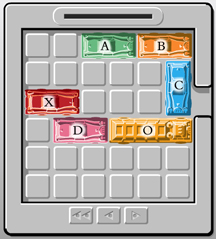
\includegraphics[scale=1.25]{resources/pictures/rushhour.jpg}
\end{center}
\end{figure}

\section{Vraag}
Rush hour is een schuifpuzzel die een verkeersopstopping voorstelt. Het doel is om de rode auto (X) uit het verkeer te krijgen in zo weinig mogelijk zetten. De andere auto's staan in de weg en elke auto kan enkel vooruit en achteruit bewegen. Auto's mogen meerdere vakjes per keer verschuiven maar er mag maar \'e\'en auto per zet verplaatst worden.\\\\
We kunnen het zoeken naar een oplossing modelleren met behulp van een graaf, waarin elke stand een knoop is en elke mogelijke zet een boog. De eindtoestand waar we dan naar op zoek gaan is een stand van het bord waarin de rode auto zich buiten het bord bevindt.

\subsection{Eindtoestand} De begintoestand is gegeven in figuur \ref{rushour}. De eindtoestand is een toestand waarin de rode auto zich buiten het bord bevindt. 

\subsection{Kostfunctie}De kostfunctie voor het A* algoritme is een belangrijke parameter. De kost van een toestand beschrijven we als het aantal vakjes dat alle autootjes in totaal verplaatst zijn om tot de huidige toestand te komen. We zouden kunnen opteren voor het aantal zetten dat nodig is om in de huidige toestand te komen als kostfunctie. Deze functie maakt minder onderscheid tussen goede en slechte toestanden en zal het probleem dus minder snel oplossen.
5
\subsection{Heuristische functie} De heuristische functie is een volgende belangrijke parameter voor het A* algoritme. Als heuristiek kiezen we het kleinste aantal auto's dat onbeweeglijk in de weg staat van de rode auto. We weten zeker dat dit een onderschatting is voor de totale kost omdat minstens al die auto's aan de kant moeten gezet worden. Als heuristiek kunnen we ook
\footnote{We voegen hier nog één aan toe, omdat doeltoestanden dan precies één hebben als heuristische waarde en omdat de heuristische waarde van een toestand dan heel makkelijk intu\"itief te zien is. bvb: De heuristische waarde van de root is $3$ want $C$ staat in de weg van de rode auto en om $C$ te verplaatsen moeten er minstens $2$ auto's verplaatst worden, namelijk $A$ en $B$ of $O$ en $D$.}.

\section{Modeloplossing}
De volledige oplossing voor dit probleem is sneller uit te leggen aan de hand van een rush-hour spelbord dan op papier. Dit probleem is echter een prachtig voorbeeld van hoe uiteenlopend de toepassingen van A* zijn. Daarom zal ik elk aspect van A* uit de oplossing eens volledig uitwerken maar niet elke keer. Ik zal het probleem dus niet volledig oplossen, maar wel zo veel als nodig. Het volledige A* algoritme bevindt zich nog eens in de appendix (\ref{A*}).\\\\
De volgende tabel stelt de begintoestand voor. Deze toestand is de wortel die initieel in de rij staat.
\begin{center}
$root = $
\begin{tabular}{| c | c | c | c | c | c |}
\hline
   &   & A & A & B & B \\ \hline
   &   &   &   &   & C \\ \hline
 X & X &   &   &   & C \\ \hline
   & D & D & O & O & O \\ \hline
   &   &   &   &   &   \\ \hline
   &   &   &   &   &   \\
\hline
\end{tabular}
\end{center}
We zullen in de uitwerking spreken over de $f$ functie. Deze definieren we als volgt.
\[
f(pad) = cost(pad) + heuristiek(einde(pad))
\]

\subsection{Iteratie 1}
We starten nu de while-lus van het A* algoritme. We expanderen alle mogelijke toestanden die in 1 zet bereikbaar zijn vanaf de begintoestand. Die toestanden zetten we allemaal in de rij. We expanderen de nodes in volgorde van het alfabet en altijd de mogelijkheid waarin het autootje de grootste afstand aflegt eerst.

\begin{center}
$T_{11} = $
\scalebox{0.5}{
\begin{tabular}{| p{0.3cm} | p{0.3cm} | p{0.3cm} | p{0.3cm} | p{0.3cm} | p{0.3cm} |}
\hline
 A & A &   &   & B & B \\ \hline
   &   &   &   &   & C \\ \hline
 X & X &   &   &   & C \\ \hline
   & D & D & O & O & O \\ \hline
   &   &   &   &   &   \\ \hline
   &   &   &   &   &   \\
\hline
\end{tabular}}
$T_{12} = $
\scalebox{0.5}{
\begin{tabular}{| p{0.3cm} | p{0.3cm} | p{0.3cm} | p{0.3cm} | p{0.3cm} | p{0.3cm} |}
\hline
   & A & A &   & B & B \\ \hline
   &   &   &   &   & C \\ \hline
 X & X &   &   &   & C \\ \hline
   & D & D & O & O & O \\ \hline
   &   &   &   &   &   \\ \hline
   &   &   &   &   &   \\
\hline
\end{tabular}}
$T_{13} = $
\scalebox{0.5}{
\begin{tabular}{| p{0.3cm} | p{0.3cm} | p{0.3cm} | p{0.3cm} | p{0.3cm} | p{0.3cm} |}
\hline
   &   & A & A & B & B \\ \hline
   &   &   &   &   & C \\ \hline
 X & X &   &   &   & C \\ \hline
 D & D &   & O & O & O \\ \hline
   &   &   &   &   &   \\ \hline
   &   &   &   &   &   \\
\hline
\end{tabular}}
\end{center}

\begin{center}
$T_{14} = $
\scalebox{0.5}{
\begin{tabular}{| p{0.3cm} | p{0.3cm} | p{0.3cm} | p{0.3cm} | p{0.3cm} | p{0.3cm} |}
\hline
   &   & A & A & B & B \\ \hline
   &   &   &   &   & C \\ \hline
   &   &   & X & X & C \\ \hline
   & D & D & O & O & O \\ \hline
   &   &   &   &   &   \\ \hline
   &   &   &   &   &   \\
\hline
\end{tabular}}
$T_{15} = $
\scalebox{0.5}{
\begin{tabular}{| p{0.3cm} | p{0.3cm} | p{0.3cm} | p{0.3cm} | p{0.3cm} | p{0.3cm} |}
\hline
   &   & A & A & B & B \\ \hline
   &   &   &   &   & C \\ \hline
   &   & X & X &   & C \\ \hline
   & D & D & O & O & O \\ \hline
   &   &   &   &   &   \\ \hline
   &   &   &   &   &   \\
\hline
\end{tabular}}
$T_{16} = $
\scalebox{0.5}{
\begin{tabular}{| p{0.3cm} | p{0.3cm} | p{0.3cm} | p{0.3cm} | p{0.3cm} | p{0.3cm} |}
\hline
   &   & A & A & B & B \\ \hline
   &   &   &   &   & C \\ \hline
   & X & X &   &   & C \\ \hline
   & D & D & O & O & O \\ \hline
   &   &   &   &   &   \\ \hline
   &   &   &   &   &   \\
\hline
\end{tabular}}
\end{center}
Geen enkele van deze paden naar deze toestanden vormt een cyclus in de zoekruimte De rij moet nu nog gesorteerd worden op de $f$ functie. Aangezien elke zet dezelfde kost heeft, namelijk $1$, is dat sorteren equivalent aan het sorteren op de heuristische waarde van elke toestand.
\[
\begin{array}{c c}
f(T_{11}) &= 2 + 2 = 4\\
f(T_{12}) &= 1 + 2 = 3\\
f(T_{13}) &= 1 + 2 = 3\\
f(T_{14}) &= 3 + 3 = 6\\
f(T_{15}) &= 2 + 3 = 5\\
f(T_{16}) &= 1 + 3 = 4\\
\end{array}
\]
De rij ziet er na deze stap als volgt uit.
\[
Q_1 = \{T_{12}, T_{13}, T_{11}, T_{16}, T_{15}, T_{14}\}
\]
\subsection{Iteratie 2}
Om de volgende iteratie te beginnen, halen we het element met de kleinste $f$-waarde uit de rij (het eerste element). In dit geval is dit $T_{12}$. We expanderen deze toestand en verkrijgen de volgende mogelijke toestanden.
\begin{center}
$T_{21} = $
\scalebox{0.5}{
\begin{tabular}{| p{0.3cm} | p{0.3cm} | p{0.3cm} | p{0.3cm} | p{0.3cm} | p{0.3cm} |}
\hline
   &   & A & A & B & B \\ \hline
   &   &   &   &   & C \\ \hline
 X & X &   &   &   & C \\ \hline
   & D & D & O & O & O \\ \hline
   &   &   &   &   &   \\ \hline
   &   &   &   &   &   \\
\hline
\end{tabular}}
$T_{22} = $
\scalebox{0.5}{
\begin{tabular}{| p{0.3cm} | p{0.3cm} | p{0.3cm} | p{0.3cm} | p{0.3cm} | p{0.3cm} |}
\hline
 A & A &   &   & B & B \\ \hline
   &   &   &   &   & C \\ \hline
 X & X &   &   &   & C \\ \hline
   & D & D & O & O & O \\ \hline
   &   &   &   &   &   \\ \hline
   &   &   &   &   &   \\
\hline
\end{tabular}}
$T_{23} = $
\scalebox{0.5}{
\begin{tabular}{| p{0.3cm} | p{0.3cm} | p{0.3cm} | p{0.3cm} | p{0.3cm} | p{0.3cm} |}
\hline
   & A & A & B & B &   \\ \hline
   &   &   &   &   & C \\ \hline
 X & X &   &   &   & C \\ \hline
   & D & D & O & O & O \\ \hline
   &   &   &   &   &   \\ \hline
   &   &   &   &   &   \\
\hline
\end{tabular}}
\end{center}
\begin{center}
$T_{24} = $
\scalebox{0.5}{
\begin{tabular}{| p{0.3cm} | p{0.3cm} | p{0.3cm} | p{0.3cm} | p{0.3cm} | p{0.3cm} |}
\hline
   & A & A &   & B & B \\ \hline
   &   &   &   &   & C \\ \hline
 X & X &   &   &   & C \\ \hline
 D & D &   & O & O & O \\ \hline
   &   &   &   &   &   \\ \hline
   &   &   &   &   &   \\
\hline
\end{tabular}}
$T_{25} = $
\scalebox{0.5}{
\begin{tabular}{| p{0.3cm} | p{0.3cm} | p{0.3cm} | p{0.3cm} | p{0.3cm} | p{0.3cm} |}
\hline
   & A & A &   & B & B \\ \hline
   &   &   &   &   & C \\ \hline
   & X & X &   &   & C \\ \hline
   & D & D & O & O & O \\ \hline
   &   &   &   &   &   \\ \hline
   &   &   &   &   &   \\
\hline
\end{tabular}}
$T_{26} = $
\scalebox{0.5}{
\begin{tabular}{| p{0.3cm} | p{0.3cm} | p{0.3cm} | p{0.3cm} | p{0.3cm} | p{0.3cm} |}
\hline
   & A & A &   & B & B \\ \hline
   &   &   &   &   & C \\ \hline
   &   & X & X &   & C \\ \hline
   & D & D & O & O & O \\ \hline
   &   &   &   &   &   \\ \hline
   &   &   &   &   &   \\
\hline
\end{tabular}}
\end{center}
\begin{center}
$T_{27} = $
\scalebox{0.5}{
\begin{tabular}{| p{0.3cm} | p{0.3cm} | p{0.3cm} | p{0.3cm} | p{0.3cm} | p{0.3cm} |}
\hline
   & A & A &   & B & B \\ \hline
   &   &   &   &   & C \\ \hline
   &   &   & X & X & C \\ \hline
   & D & D & O & O & O \\ \hline
   &   &   &   &   &   \\ \hline
   &   &   &   &   &   \\
\hline
\end{tabular}}
\end{center}
Wanneer we nu deze nieuwe toestanden nakijken om te zien of er geen cycli zijn gevormd, zien we dat $T_{21} = root$. Dit betekent dat we $T_{21}$ al mogen verwijderen. We zetten de andere toestanden bij in de rij en sorteren deze weer.
\[
\begin{array}{c c}
f(T_{22}) &= 2+ 2 = 4\\
f(T_{23}) &= 2+ 1 = 3\\
f(T_{24}) &= 2+ 2 = 4\\
f(T_{25}) &= 2+ 2 = 4\\
f(T_{26}) &= 3+ 2 = 5\\
f(T_{27}) &= 4+ 2 = 6\\
\end{array}
\]
We verkrijgen dan de volgende rij.
\[
Q_2 = \{T_{23}, T_{12}, T_{13}, T_{22}, T_{24}, T_{25}, T_{11}, T_{16}, T_{26}, T_{15}, T_{27}, T_{14}\}
\]

\subsection{Iteratie 3}
Het volgende element dat we moeten expanderen is $T_{23}$. Wanneer we dit doen zien we dat we al vrij dicht bij de gewenste uitkomst komen. De volgende toestanden zijn de toestanden die bereikbaar zijn vanuit $T_{23}$.
\begin{center}
$T_{31} = $
\scalebox{0.5}{
\begin{tabular}{| p{0.3cm} | p{0.3cm} | p{0.3cm} | p{0.3cm} | p{0.3cm} | p{0.3cm} |}
\hline
 A & A &   & B & B &   \\ \hline
   &   &   &   &   & C \\ \hline
 X & X &   &   &   & C \\ \hline
   & D & D & O & O & O \\ \hline
   &   &   &   &   &   \\ \hline
   &   &   &   &   &   \\
\hline
\end{tabular}}
$T_{32} = $
\scalebox{0.5}{
\begin{tabular}{| p{0.3cm} | p{0.3cm} | p{0.3cm} | p{0.3cm} | p{0.3cm} | p{0.3cm} |}
\hline
   & A & A &   & B & B \\ \hline
   &   &   &   &   & C \\ \hline
 X & X &   &   &   & C \\ \hline
   & D & D & O & O & O \\ \hline
   &   &   &   &   &   \\ \hline
   &   &   &   &   &   \\
\hline
\end{tabular}}
$T_{33} = $
\scalebox{0.5}{
\begin{tabular}{| p{0.3cm} | p{0.3cm} | p{0.3cm} | p{0.3cm} | p{0.3cm} | p{0.3cm} |}
\hline
   & A & A & B & B & C \\ \hline
   &   &   &   &   & C \\ \hline
 X & X &   &   &   &   \\ \hline
   & D & D & O & O & O \\ \hline
   &   &   &   &   &   \\ \hline
   &   &   &   &   &   \\
\hline
\end{tabular}}
\end{center}
\begin{center}
$T_{34} = $
\scalebox{0.5}{
\begin{tabular}{| p{0.3cm} | p{0.3cm} | p{0.3cm} | p{0.3cm} | p{0.3cm} | p{0.3cm} |}
\hline
   & A & A & B & B &   \\ \hline
   &   &   &   &   & C \\ \hline
 X & X &   &   &   & C \\ \hline
 D & D &   & O & O & O \\ \hline
   &   &   &   &   &   \\ \hline
   &   &   &   &   &   \\
\hline
\end{tabular}}
$T_{35} = $
\scalebox{0.5}{
\begin{tabular}{| p{0.3cm} | p{0.3cm} | p{0.3cm} | p{0.3cm} | p{0.3cm} | p{0.3cm} |}
\hline
   & A & A & B & B &   \\ \hline
   &   &   &   &   & C \\ \hline
   & X & X &   &   & C \\ \hline
   & D & D & O & O & O \\ \hline
   &   &   &   &   &   \\ \hline
   &   &   &   &   &   \\
\hline
\end{tabular}}
$T_{36} = $
\scalebox{0.5}{
\begin{tabular}{| p{0.3cm} | p{0.3cm} | p{0.3cm} | p{0.3cm} | p{0.3cm} | p{0.3cm} |}
\hline
   & A & A & B & B &   \\ \hline
   &   &   &   &   & C \\ \hline
   &   & X & X &   & C \\ \hline
   & D & D & O & O & O \\ \hline
   &   &   &   &   &   \\ \hline
   &   &   &   &   &   \\
\hline
\end{tabular}}
\end{center}
\begin{center}
$T_{37} = $
\scalebox{0.5}{
\begin{tabular}{| p{0.3cm} | p{0.3cm} | p{0.3cm} | p{0.3cm} | p{0.3cm} | p{0.3cm} |}
\hline
   & A & A & B & B &   \\ \hline
   &   &   &   &   & C \\ \hline
   &   &   & X & X & C \\ \hline
   & D & D & O & O & O \\ \hline
   &   &   &   &   &   \\ \hline
   &   &   &   &   &   \\
\hline
\end{tabular}}
\end{center}
We zien dat $T_{32}$ een cyclus vormt met $T_{12}$. Deze toestand mag dus al verwijderd worden.
\[
\begin{array}{c c}
f(T_{31}) &= 3 + 1 = 4\\
f(T_{33}) &= 3 + 0 = 3\\
f(T_{34}) &= 3 + 1 = 4\\
f(T_{35}) &= 3 + 1 = 4\\
f(T_{36}) &= 4 + 1 = 5\\
f(T_{37}) &= 5 + 1 = 6\\
\end{array}
\]
Als we deze toestanden toevoegen aan de rij en deze opnieuw sorteren, krijgen we de volgende rij.
\[
Q_3 = \{T_{33}, T_{13}, T_{31}, T_{34}, T_{35}, T_{22}, T_{24}, T_{25}, T_{11}, T_{16}, T_{36}, T_{26}, T_{15}, T_{37}, T_{27}, T_{14}\}
\]

\subsection{Iteratie 4}
De volgende toestand die we expanderen is $T_{33}$.
\begin{center}
$T_{41} = $
\scalebox{0.5}{
\begin{tabular}{| p{0.3cm} | p{0.3cm} | p{0.3cm} | p{0.3cm} | p{0.3cm} | p{0.3cm} |}
\hline
 A & A &   & B & B & C \\ \hline
   &   &   &   &   & C \\ \hline
 X & X &   &   &   &   \\ \hline
   & D & D & O & O & O \\ \hline
   &   &   &   &   &   \\ \hline
   &   &   &   &   &   \\
\hline
\end{tabular}}
$T_{42} = $
\scalebox{0.5}{
\begin{tabular}{| p{0.3cm} | p{0.3cm} | p{0.3cm} | p{0.3cm} | p{0.3cm} | p{0.3cm} |}
\hline
   & A & A & B & B &   \\ \hline
   &   &   &   &   & C \\ \hline
 X & X &   &   &   & C \\ \hline
   & D & D & O & O & O \\ \hline
   &   &   &   &   &   \\ \hline
   &   &   &   &   &   \\
\hline
\end{tabular}}
$T_{43} = $
\scalebox{0.5}{
\begin{tabular}{| p{0.3cm} | p{0.3cm} | p{0.3cm} | p{0.3cm} | p{0.3cm} | p{0.3cm} |}
\hline
   & A & A & B & B & C \\ \hline
   &   &   &   &   & C \\ \hline
 X & X &   &   &   &   \\ \hline
 D & D &   & O & O & O \\ \hline
   &   &   &   &   &   \\ \hline
   &   &   &   &   &   \\
\hline
\end{tabular}}
\end{center}
\begin{center}
$T_{44} = $
\scalebox{0.5}{
\begin{tabular}{| p{0.3cm} | p{0.3cm} | p{0.3cm} | p{0.3cm} | p{0.3cm} | p{0.3cm} |}
\hline
   & A & A & B & B & C \\ \hline
   &   &   &   &   & C \\ \hline
   & X & X &   &   &   \\ \hline
   & D & D & O & O & O \\ \hline
   &   &   &   &   &   \\ \hline
   &   &   &   &   &   \\
\hline
\end{tabular}}
$T_{45} = $
\scalebox{0.5}{
\begin{tabular}{| p{0.3cm} | p{0.3cm} | p{0.3cm} | p{0.3cm} | p{0.3cm} | p{0.3cm} |}
\hline
   & A & A & B & B & C \\ \hline
   &   &   &   &   & C \\ \hline
   &   & X & X &   &   \\ \hline
   & D & D & O & O & O \\ \hline
   &   &   &   &   &   \\ \hline
   &   &   &   &   &   \\
\hline
\end{tabular}}
$T_{46} = $
\scalebox{0.5}{
\begin{tabular}{| p{0.3cm} | p{0.3cm} | p{0.3cm} | p{0.3cm} | p{0.3cm} | p{0.3cm} |}
\hline
   & A & A & B & B & C \\ \hline
   &   &   &   &   & C \\ \hline
   &   &   & X & X &   \\ \hline
   & D & D & O & O & O \\ \hline
   &   &   &   &   &   \\ \hline
   &   &   &   &   &   \\
\hline
\end{tabular}}
\end{center}
\begin{center}
$T_{47} = $
\scalebox{0.5}{
\begin{tabular}{| p{0.3cm} | p{0.3cm} | p{0.3cm} | p{0.3cm} | p{0.3cm} | p{0.3cm} |}
\hline
   & A & A & B & B & C \\ \hline
   &   &   &   &   & C \\ \hline
   &   &   &   & X & X \\ \hline
   & D & D & O & O & O \\ \hline
   &   &   &   &   &   \\ \hline
   &   &   &   &   &   \\
\hline
\end{tabular}}
$T_{48} = $
\scalebox{0.5}{
\begin{tabular}{| p{0.3cm} | p{0.3cm} | p{0.3cm} | p{0.3cm} | p{0.3cm} | p{0.3cm} |}
\hline
   & A & A & B & B & C \\ \hline
   &   &   &   &   & C \\ \hline
   &   &   &   &   & X \\ \hline
   & D & D & O & O & O \\ \hline
   &   &   &   &   &   \\ \hline
   &   &   &   &   &   \\
\hline
\end{tabular}}
$T_{49} = $
\scalebox{0.5}{
\begin{tabular}{| p{0.3cm} | p{0.3cm} | p{0.3cm} | p{0.3cm} | p{0.3cm} | p{0.3cm} |}
\hline
   & A & A & B & B & C \\ \hline
   &   &   &   &   & C \\ \hline
   &   &   &   &   &   \\ \hline
   & D & D & O & O & O \\ \hline
   &   &   &   &   &   \\ \hline
   &   &   &   &   &   \\
\hline
\end{tabular}}
\end{center}
We zien dat $T_{42}$ een cyclus vormt met $T_{23}$ en verwijderen daarom deze toestand. Elk van de overgebleven toestanden heeft als heuristische waarde $h(T_{4i}) = 0$. De $f$-waarde van deze toestanden is dus $f(T_{4i}) = 4$.
We voegen ten slotte deze toestanden toe aan de rij.
\begin{center}
\[
Q_4 = \{T_{13}, T_{41}, T_{43}, T_{47}, T_{45}, T_{46}, T_{47}, T_{48}, T_{49}, T_{31}, T_{34},
\]
\[
T_{35}, T_{22}, T_{24}, T_{25}, T_{11}, T_{16}, T_{36}, T_{26}, T_{15}, T_{37}, T_{27}, T_{14}\}
\]
\end{center}
We zien nu dat er een doeltoestand in de rij staat, namelijk $T_{49}$, maar A* zal nog niet stoppen, want $T_{49}$ staat nog niet vooraan de lijst.

\subsection{Verdere uitwerking}
De verdere uitwerking van de oplossing zal ik hier niet volledig opschrijven, maar beschrijven.\\\\
Eigen aan dit probleem is dat er in de latere iteraties zeer veel cycli zullen worden gevormd, omdat het aantal mogelijke staten eindig en zelfs vrij klein is.
Als we naar de rij kijken, na de 4$^{de}$ iteratie, zien we dat de doeloplossing die er na de 4$^{de}$ iteratie in zit, op de 9$^de$ plaats staat. Vanaf nu zal A* enkel nog oplossingen vinden die ofwel beter zijn dan het pad naar $T_{49}$, ofwel slechter zijn, en dus worden verwijderd. In deze opgave is het toevallig zo dat er twee even lange paden zijn naar een eindtoestand. A* zal ze dus zeker alle twee gevonden hebben op een bepaald moment. Het algoritme zal één van de twee paden verwijderen uit de rij. We weten dus dat A*, in dit specifiek geval, nog minstens 9 iteraties zal voltooien voordat het tot een oplossing komt. Bovendien zijn er paden die nooit zullen bekeken worden. Hiervan is het pad met $T_{14}$ een voorbeeld.\\\\
Elk aspect van A* is nu aan bod gekomen.
\begin{itemize}
\item Kostfunctie
\item Heuristische functie
\item Het verwijderen van cycli
\item Het verwijderen van langere paden naar het doel
\item Nooit geselecteerde knopen.
\end{itemize}

\end{document}